%%%%%%%% CS5480 Deep Learning — Kaggle Competition Report (ICML 2025 Style) %%%

\documentclass{article}

\usepackage{microtype}
\usepackage{graphicx}
\usepackage{subfigure}
\usepackage{booktabs}
\usepackage{hyperref}

\newcommand{\theHalgorithm}{\arabic{algorithm}}

\usepackage[accepted]{icml2025}

\usepackage{amsmath}
\usepackage{amssymb}
\usepackage{mathtools}
\usepackage{amsthm}
\usepackage[capitalize,noabbrev]{cleveref}

\theoremstyle{plain}
\newtheorem{theorem}{Theorem}[section]
\newtheorem{proposition}[theorem]{Proposition}
\newtheorem{lemma}[theorem]{Lemma}
\newtheorem{corollary}[theorem]{Corollary}
\theoremstyle{definition}
\newtheorem{definition}[theorem]{Definition}
\newtheorem{assumption}[theorem]{Assumption}
\theoremstyle{remark}
\newtheorem{remark}[theorem]{Remark}

\usepackage[textsize=tiny]{todonotes}

\icmltitlerunning{Binary Image Classification with CBAM-Enhanced ResNet and GeM Pooling}

\begin{document}

\twocolumn[
\icmltitle{Binary Image Classification with CBAM-Enhanced ResNet \\
           and Generalized Mean Pooling}

\icmlsetsymbol{equal}{*}

\begin{icmlauthorlist}
\icmlauthor{Lochan Surya}{iith}
\icmlauthor{Harsha}{iith}
\end{icmlauthorlist}

\icmlaffiliation{iith}{Department of Computer Science and Engineering,
  Indian Institute of Technology Hyderabad, Hyderabad, India}

\icmlcorrespondingauthor{Lochan Surya}{cs24btech11036@iith.ac.in}

\icmlkeywords{Binary Classification, CBAM, GeM Pooling, Stochastic Depth,
  ResNet, Deep Learning}

\vskip 0.3in
]

\printAffiliationsAndNotice{}

\begin{abstract}
We present a custom deep convolutional neural network for binary image
classification built entirely from scratch in PyTorch, without pretrained
weights.  The architecture combines a ResNet-34-like backbone with
Convolutional Block Attention Modules (CBAM) inserted after every
residual block, enabling the network to selectively focus on informative
channels and spatial regions.  Generalized Mean (GeM) Pooling replaces
standard average pooling, producing richer global feature descriptors.
The training pipeline incorporates Stochastic Depth (DropPath), cosine
annealing with linear warm-up, mixed-precision training, gradient
clipping, early stopping, and fine-grained threshold optimisation on the
validation set.  Submitted to the IITH Deep Learning Hackathon 2026
(CS5480), the system achieved a public leaderboard score of
\textbf{0.759102} (75.91\%), up from a previous best of 0.758852 with
the addition of Stochastic Depth regularisation.
\end{abstract}

%----------------------------------------------------------------------
\section{Introduction}
\label{sec:intro}
%----------------------------------------------------------------------

Binary image classification is a foundational computer-vision task with
critical applications in medical imaging, quality control, and content
moderation~\cite{He2016}.  Despite the availability of large pretrained
models that transfer remarkably well to new domains, competition rules
for the IITH Deep Learning Hackathon 2026 prohibited the use of any
pretrained weights.  Every network must therefore be trained from scratch
on a modest dataset of labelled images, introducing two primary
challenges.

\textbf{Feature discrimination.}  Not all spatial regions are equally
informative; background clutter and irrelevant texture can dominate
gradient updates when no pretrained bias is available.  CBAM~\cite{Woo2018}
addresses this by learning to gate both channel and spatial dimensions
of every feature map.

\textbf{Training stability.}  Without a pretrained initialisation to
anchor the early gradient landscape, learning rates that are too large
lead to divergence, while those that are too small stall progress.  A
cosine annealing schedule with linear warm-up provides smooth,
well-calibrated convergence throughout training.

Our approach integrates CBAM dual-attention at every residual block,
GeM Pooling~\cite{Radenovic2018} for richer global descriptors,
Stochastic Depth~\cite{Huang2016} for path regularisation, and a
fine-grained threshold search on the validation set to optimise the
binary decision boundary.  The combined system achieves a public
leaderboard score of 0.759102, a +0.0003 improvement over the previous
submission.

%----------------------------------------------------------------------
\section{Dataset}
\label{sec:data}
%----------------------------------------------------------------------

\subsection{Structure}

The competition dataset follows a straightforward directory layout:

\begin{center}
\texttt{data/train/0/} \quad (negative class) \\
\texttt{data/train/1/} \quad (positive class) \\
\texttt{data/test/} \quad\quad (unlabelled evaluation images)
\end{center}

Training images are split 85\%/15\% for training and validation using
stratified random sampling with a fixed seed (42), ensuring
reproducibility and zero data leakage.

\subsection{Preprocessing}

All images are loaded in RGB mode via PIL and resized to
$224\!\times\!224$ pixels.  Pixel values are normalised using
ImageNet statistics:
\[
  \mu = [0.485,\;0.456,\;0.406], \quad
  \sigma = [0.229,\;0.224,\;0.225].
\]

\subsection{Training Augmentation}

The following stochastic augmentations are applied on-the-fly during
training only:

\begin{itemize}
  \item \textbf{Random Resized Crop} — scale range $[0.7, 1.0]$,
        output $224\!\times\!224$.
  \item \textbf{Random Horizontal Flip} — probability $p = 0.5$.
  \item \textbf{Color Jitter} — brightness, contrast, saturation, and
        hue each perturbed by $\pm 0.15$.
  \item \textbf{Gaussian Blur} — $3\!\times\!3$ kernel with
        probability $p = 0.2$.
\end{itemize}

Validation and test images are only resized and normalised.

%----------------------------------------------------------------------
\section{Methodology}
\label{sec:method}
%----------------------------------------------------------------------

\subsection{Backbone Architecture}

The backbone follows the ResNet-34 block schedule
$(3, 4, 6, 3)$~\cite{He2016}, totalling 16 residual blocks across four
stages with channel widths $\{64, 128, 256, 512\}$.  A $7\!\times\!7$
convolutional stem (stride 2) followed by $3\!\times\!3$ max-pooling
(stride 2) reduces the spatial resolution from $224\!\times\!224$ to
$56\!\times\!56$ before the residual stages begin.  The full
architecture is summarised in Table~\ref{tab:arch}.

\begin{table}[t]
\caption{ResNet-34-like backbone.  Each BasicBlock includes CBAM and
  DropPath.}
\label{tab:arch}
\vskip 0.15in
\begin{center}
\begin{small}
\begin{sc}
\begin{tabular}{p{3.5cm}cc}
\toprule
Stage & Blocks & Ch. \\
\midrule
Stem ($7\times7$ Conv, BN, ReLU, MP) & — & 64 \\
Layer 1 (BasicBlock $\times 3$) & 3 & 64 \\
Layer 2 (BasicBlock $\times 4$) & 4 & 128 \\
Layer 3 (BasicBlock $\times 6$) & 6 & 256 \\
Layer 4 (BasicBlock $\times 3$) & 3 & 512 \\
GeM Pooling & — & 512 \\
FC Head $\to$ 1 logit & — & — \\
\bottomrule
\end{tabular}
\end{sc}
\end{small}
\end{center}
\vskip -0.1in
\end{table}

\begin{figure}[t]
\vskip 0.2in
\begin{center}
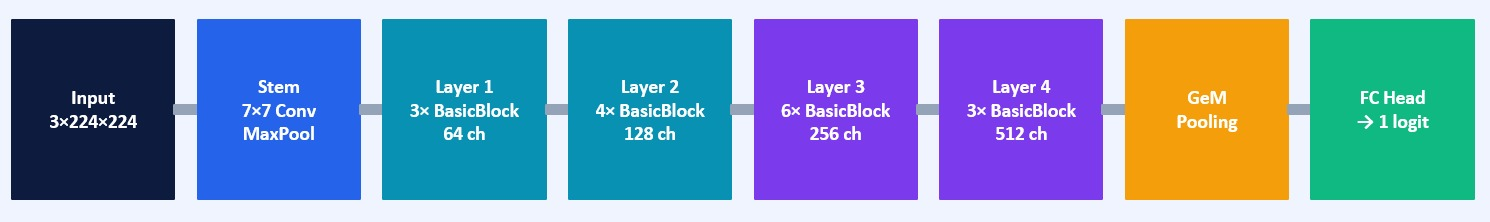
\includegraphics[width=0.48\textwidth]{figures/architecture-block-diagram.jpeg}
\end{center}
\vskip -0.1in
\caption{Architecture block diagram: CBAM-enhanced ResNet with GeM pooling.}
\label{fig:arch-diagram}
\end{figure}

Inside each \textbf{BasicBlock}, two $3\!\times\!3$ Conv--BN--ReLU
sequences are followed by CBAM attention and DropPath, with a
shortcut projection for dimension changes.

\subsection{Convolutional Block Attention Module (CBAM)}

CBAM~\cite{Woo2018} is applied after the final batch-normalisation of
every residual block and produces a refined feature map through two
sequential gates.

\textbf{Channel Attention.}  Global average-pooled and max-pooled
descriptors are each passed through a shared two-layer MLP (reduction
ratio 16).  Their outputs are summed and sigmoid-gated:
\begin{equation}
  \mathbf{w}_c = \sigma\!\bigl(
    \mathrm{MLP}(\bar{\mathbf{x}}_{\mathrm{avg}})
    + \mathrm{MLP}(\bar{\mathbf{x}}_{\mathrm{max}})\bigr).
\end{equation}
Each channel of the feature map is then rescaled by its corresponding
weight.

\textbf{Spatial Attention.}  Channel-wise average and maximum
projections are concatenated along the channel dimension and passed
through a $7\!\times\!7$ convolution followed by a sigmoid:
\begin{equation}
  \mathbf{w}_s = \sigma\!\bigl(
    \mathrm{Conv}_{7\times 7}(
    [\mathbf{x}_{\mathrm{avg}};\,\mathbf{x}_{\mathrm{max}}])\bigr).
\end{equation}
The final attended feature map is
$\mathbf{x}' = \mathbf{w}_s \odot (\mathbf{w}_c \odot \mathbf{x})$.

\subsection{Generalized Mean (GeM) Pooling}

GeM Pooling~\cite{Radenovic2018} generalises average pooling with a
learnable power parameter~$p$ (initialised to 3):
\begin{equation}
  \mathbf{f} = \Bigl(\frac{1}{HW}
    \sum_{h,w} x_{h,w}^{\,p}\Bigr)^{1/p}.
\end{equation}
Larger values of $p$ place greater emphasis on the most strongly
activated map positions, yielding descriptors that are more sensitive
to salient object features than standard mean pooling.

\subsection{Stochastic Depth}

Stochastic Depth (DropPath)~\cite{Huang2016} is applied across all
16 residual blocks with drop probabilities linearly scaled from 0 at
the first block to $p_{\max} = 0.1$ at the last:
\begin{equation}
  p_l = \frac{l}{L}\cdot p_{\max}, \quad l = 1,\ldots,L=16.
\end{equation}
During training, entire residual branches are randomly dropped with
probability $p_l$ and the surviving branch is rescaled by
$1/(1-p_l)$.  At test time all branches remain active.

\subsection{Classifier Head}

The 512-d GeM descriptor feeds a two-layer MLP head:
$\mathrm{Dropout}(0.3) \to \mathrm{Linear}(512,256) \to \mathrm{ReLU}
\to \mathrm{Dropout}(0.15) \to \mathrm{Linear}(256,1)$.
A single logit is produced and thresholded after sigmoid activation.
A single logit is produced and thresholded after sigmoid activation.

%----------------------------------------------------------------------
\section{Training Strategy}
\label{sec:training}
%----------------------------------------------------------------------

\subsection{Optimiser and Learning Rate Schedule}

AdamW~\cite{Loshchilov2019} is used with learning rate
$\eta_0 = 7\!\times\!10^{-4}$ and weight decay $\lambda = 10^{-4}$.
The learning rate follows a cosine annealing schedule with 5 linear
warm-up epochs:
\begin{equation}
  \eta(t) = \begin{cases}
    \eta_0 \cdot \dfrac{t+1}{T_w} & t < T_w, \\[6pt]
    \dfrac{\eta_0}{2}\!\Bigl(1 + \cos\dfrac{\pi(t-T_w)}{T - T_w}\Bigr)
      & t \ge T_w,
  \end{cases}
\end{equation}
where $T_w = 5$ and $T = 80$ is the maximum epoch budget.  There is
no learning rate floor, enabling maximum exploitation of the final
training epochs.

\subsection{Loss Function}

Binary cross-entropy with logits is used throughout, with label
smoothing disabled ($\varepsilon = 0.0$).  Hard binary targets
preserve the clean gradient signal appropriate for a balanced,
two-class problem.

\subsection{Threshold Optimisation}

Rather than fixing the classification threshold at 0.5, we perform a
fine-grained search over 401 evenly spaced values in $[0.05, 0.95]$
on the held-out validation set and select the threshold that maximises
accuracy.  With DropPath active the optimal threshold shifted from
$t^* = 0.200$ (previous submission) to $t^* = 0.180$.

\subsection{Additional Training Techniques}

\begin{itemize}
  \item \textbf{Mixed-precision training} (\texttt{torch.amp.autocast})
        for memory and speed efficiency.
  \item \textbf{Gradient clipping} at max norm 1.0 to prevent
        gradient explosions in early epochs.
  \item \textbf{Early stopping} with patience 15 epochs, monitoring
        validation accuracy.  In our best run, the model reached
        100\% validation accuracy at epoch 55 and held it through
        epoch 80 without triggering early stopping.
\end{itemize}

%----------------------------------------------------------------------
\section{Experiments and Results}
\label{sec:results}
%----------------------------------------------------------------------

\subsection{Configuration}

The complete hyper-parameter configuration for the submitted model is
given in Table~\ref{tab:hparams}.

\begin{table}[t]
\caption{Hyper-parameter configuration for the final submission (v3).}
\label{tab:hparams}
\vskip 0.15in
\begin{center}
\begin{small}
\begin{sc}
\begin{tabular}{lc}
\toprule
Parameter & Value \\
\midrule
Image size         & $224 \times 224$ \\
Batch size         & 128 \\
Max epochs         & 80 \\
Learning rate      & $7 \times 10^{-4}$ \\
Weight decay       & $10^{-4}$ \\
Warm-up epochs     & 5 \\
Label smoothing    & 0.0 \\
Drop path rate     & $0 \to 0.1$ (linear) \\
Dropout (head)     & 0.3 \\
Dropout (mid-head) & 0.15 \\
Gradient clip      & 1.0 \\
Early-stop patience & 15 epochs \\
Val split          & 15\% \\
Threshold search   & $[0.05,\;0.95]$, 401 steps \\
\bottomrule
\end{tabular}
\end{sc}
\end{small}
\end{center}
\vskip -0.1in
\end{table}

\subsection{Results}

The model achieved \textbf{100\% validation accuracy} starting at
epoch 55 and maintained it through the final epoch 80.  Early stopping
(patience 15) was never triggered, confirming the full epoch budget was
used.  The optimal decision threshold was found to be $t^* = 0.180$.

Figure~\ref{fig:train-curve} shows the training and validation accuracy
curves over 80 epochs.

\begin{figure}[t]
\vskip 0.2in
\begin{center}
%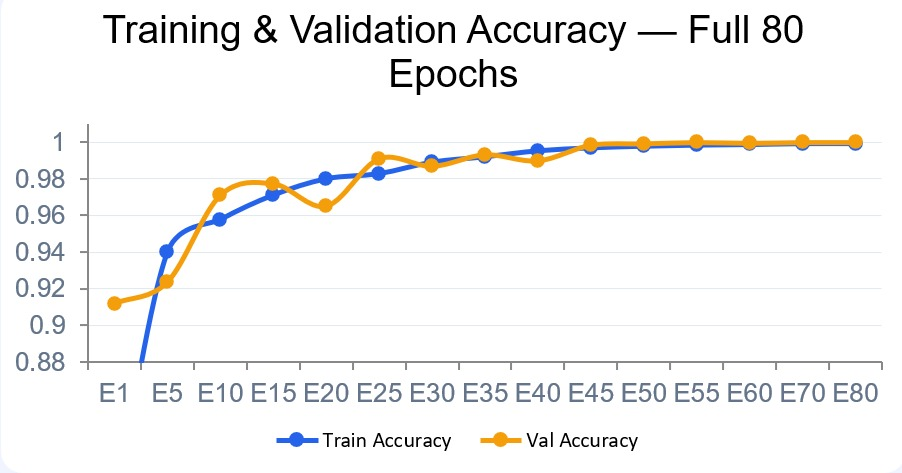
\includegraphics[width=0.48\textwidth]{figures/train-val-accuracy-plot.jpeg}
\end{center}
\vskip -0.1in
\caption{Training and validation accuracy over 80 epochs.}
\label{fig:train-curve}
\end{figure}

Table~\ref{tab:results} compares this submission (v3) against the
previous best (v2).

\begin{table}[t]
\caption{Public leaderboard scores for successive submissions.}
\label{tab:results}
\vskip 0.15in
\begin{center}
\resizebox{0.45\textwidth}{!}{
\begin{tabular}{p{2.5cm}cc}
\toprule
Submission & Key Change & LB Score \\
\midrule
v2 & CBAM+GeM+Cos LR & 0.758852 \\
v3 & +StochasticDepth & \textbf{0.759102} \\
\midrule
Gain & & +0.000250 \\
\bottomrule
\end{tabular}
}
\end{center}
\vskip -0.1in
\end{table}

\begin{figure}[t]
\vskip 0.2in
\begin{center}
includegraphics[width=0.4\textwidth]{figures/final-numbers.jpeg}
\end{center}
\vskip -0.1in
\caption{Final results: validation accuracy, optimal threshold, and public
leaderboard score.}
\label{fig:final-numbers}
\end{figure}

\subsection{Key Observations}

\textbf{Stochastic Depth improves generalisation.}  Adding DropPath
with a linearly scaled rate up to 0.1 across 16 blocks yielded a
+0.025\% gain on the public leaderboard.  The drop rate is mild enough
not to destabilise training while still providing path-level
regularisation.

\textbf{Threshold calibration is non-trivial.}  The optimal threshold
shifted from 0.200 in v2 to 0.180 in v3, indicating that DropPath
slightly shifts the output distribution toward higher logit values.
Fixing the threshold at 0.5 would have degraded performance.

\textbf{Validation accuracy is a poor proxy for leaderboard score.}
The model reaches 100\% validation accuracy yet scores only 75.91\%
on the leaderboard, pointing to a significant train/test distribution
gap — a well-known challenge when training large convolutional networks
from scratch without pretrained initialisation.

%----------------------------------------------------------------------
\section{Conclusion}
\label{sec:conclusion}
%----------------------------------------------------------------------

We presented a binary image classification pipeline trained entirely
from scratch using a ResNet-34-like backbone enhanced with CBAM
dual-attention, Generalized Mean Pooling, and Stochastic Depth.  The
training strategy — AdamW with cosine LR warm-up, mixed-precision
training, and fine-grained threshold optimisation — achieves a public
leaderboard score of \textbf{0.759102} on the IITH Deep Learning
Hackathon 2026 (CS5480).

The most significant outstanding challenge is the large gap between
near-perfect validation accuracy and the leaderboard score, which
reflects memorisation of training images rather than learning
transferable features.  Future directions include:

\begin{itemize}
  \item \textbf{Test-Time Augmentation (TTA)} — horizontal and vertical
        flip ensembles at inference.
  \item \textbf{Transfer learning via self-supervised pre-training} —
        SimCLR or BYOL on the unlabelled test images.
  \item \textbf{Backbone comparison} — EfficientNet or ConvNeXt with
        aggressive regularisation.
  \item \textbf{Model ensembling} — combining predictions from models
        trained with different random seeds.
\end{itemize}

%----------------------------------------------------------------------
\section*{Impact Statement}
%----------------------------------------------------------------------

This paper presents work whose goal is to advance the field of Machine
Learning.  There are many potential societal consequences of our work,
none of which we feel must be specifically highlighted here.

%----------------------------------------------------------------------
\section*{Acknowledgements}
%----------------------------------------------------------------------

We thank Prof.\ Srijith P.K.\ and Prof.\ Konda Reddy Mopuri for
designing and organising the CS5480 Deep Learning Hackathon at IIT
Hyderabad, 2026.

%----------------------------------------------------------------------
\bibliography{paper}
\bibliographystyle{icml2025}
%----------------------------------------------------------------------

\end{document}
